\chapter{Project Management}\label{ch:project_management}

This chapter outlines the project's management approach, including the development methodology, planning, and reflections on the process. It also considers legal and ethical issues and assesses key risks associated with the project.

\section{Methodology}
The project adopted an agile methodology, chosen for its flexibility, iterative development cycle, and emphasis on frequent customer feedback. The work involved incrementally building a series of interdependent features into vodle -- starting with a core delegation mechanism, and progressively expanding functionality to include ranked delegation, vote splitting, and finally, per-option delegation. This iterative approach allowed each new feature to build directly upon the last, ensuring ongoing compatibility and adaptability in design decisions as the system evolved.

Agile methodology was particularly suitable for this project due to the involvement of an active ``customer'' figure: Jobst Heitzig, co-supervisor and original creator of vodle. Heitzig played a crucial role in defining system expectations and guiding design decisions based on practical, real-world considerations. Regular meetings, held fortnightly with both Jobst Heitzig and Markus Brill, facilitated continuous feedback and review of progress, enabling rapid adaptation of development plans. This feedback cycle closely reflects the Agile Manifesto's principles of early and continuous delivery, as well as close collaboration between developers and stakeholders \citep{agilemanifesto2001}.

Other project management approaches, such as Waterfall, were also evaluated but ultimately dismissed due to their inherent rigidity. Although Waterfall initially appeared attractive due to clearly defined phases and comprehensive documentation at each stage, its requirement to specify the complete project scope upfront was incompatible with the evolving nature of the project. Given the shorter timeframe and the dynamic nature of feature requirements, the flexibility afforded by agile was critical to the project's success.

Scrum, one of the most widely adopted agile frameworks (used by approximately 63\% of agile teams \citep{versionone2020stateofagile}), was also considered. Its structured, sprint-based cycles, clear team roles, and structured ceremonies such as sprint planning and reviews were appealing for maintaining focused implementation and streamlined communication. However, the project's constraints -- limited availability due to academic commitments and a small team size -- made Scrum's daily stand-up meetings and fixed sprint lengths impractical. As a result, the project adopted an adapted agile approach: progress was reviewed every two weeks, effectively maintaining the advantages of frequent feedback without the constraints and scheduling pressures imposed by full Scrum ceremonies.

Each iteration of development produced a functional, testable feature that could be immediately evaluated and integrated into the broader system. This method significantly reduced the risk of late-stage integration issues and ensured steady, measurable progress throughout the project's duration. Overall, the agile methodology's iterative, feedback-oriented structure proved highly effective, meeting both the technical complexity and collaborative needs inherent in this work.
\section{Plan}

The project plan was organised into objectives (see Section \ref{ch:project_objectives}) that built on one another in sequence:

\begin{itemize}
    \item \textbf{Core Objective 1:} Implement a Core Delegation Model into Vodle.
    \item \textbf{Core Objective 2:} Implement Ranked Delegation into Vodle.
    \item \textbf{Core Objective 3:} Implement a Vote Splitting Delegation Mechanism into Vodle.
    \item \textbf{Core Objective 4:} Implement the Ability to Delegate Individual Options to Different Users.
    \item \textbf{Extension Objective 1:} Simulate Delegation Mechanisms.
\end{itemize}

This objective-led structure was well-suited to the agile approach, allowing each milestone to be treated as an iteration with a deliverable at the end. A Gantt chart (see below) was created to visualise the project timeline and to track dependencies and progress.

\begin{figure}[H]
    \centering
    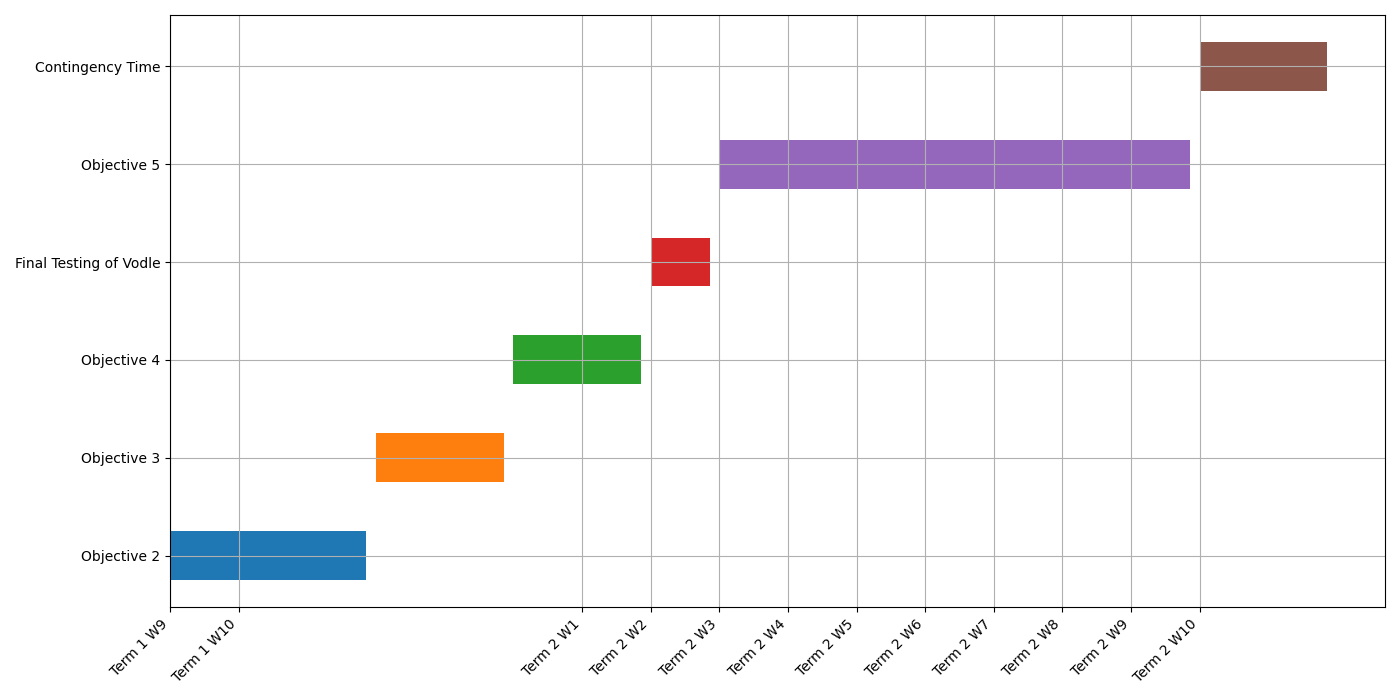
\includegraphics[width=0.8\textwidth]{../common/initial_gantt.png}
    \caption{Gantt chart illustrating the project plan from the progress report.}
    \label{fig:gantt}
\end{figure}


\section{Changes to the Project Plan}
The original project plan, illustrated in the Gantt chart (Figure~\ref{fig:gantt}), outlined a linear progression through the core objectives. However, several adjustments were made during the course of the project to reflect evolving priorities and unforeseen technical challenges.

The most significant change was the decision to de-scope the extension objective (simulating delegation mechanisms). This was prompted by two main factors. First, implementing the core objectives proved more technically demanding than initially anticipated -- particularly ranked delegation and vote splitting. These challenges required more time and attention than expected, leaving limited capacity to complete the extension objective without compromising the quality of the core deliverables.

Second, during the background research phase, it became clear that similar investigations into delegation behaviour had already been conducted -- most notably by \citet{brill_liquid_2021}. Although their study did not use agent based modelling, instead using networks from synthetic and real-world networks (such as partial networks from Facebook, Twitter, Slashdot, etc.), it provided a comprehensive empirical evaluation of ranked delegation rules using various metrics such as maximum vote path length, average vote path rank, the number of isolated voters (voters without a delegation path) and many more.

Given the depth and relevance of these findings, replicating the analysis through agent-based modelling, especially within the project's limited timeframe, was deemed unnecessary. Instead, the project focused on fully delivering and refining the core objectives, which aligned more directly with vodle's platform goals and would have a better impact on the user experience of vodle.

A second change involved reversing the development order of objectives 3 and 4. Originally, objective 3 (vote splitting) was scheduled to follow objective 2. However, during the Christmas development period, it became clear that objective 4 (per-option delegation) could be completed more quickly and required fewer algorithmic dependencies. To maintain development momentum, objective 4 was brought forward.

This adjustment helped mitigate project risk. Objective 4 involved minimal changes to the database schema and integrated easily with UI components developed for earlier objectives. In contrast, objective 3 introduced more complex computational logic and performance concerns, which demanded additional design, testing and changes to the database. Tackling objective 4 earlier helped avoid potential cascading delays and ensured a smoother integration process later in development.

\section{Risk Assessment - TODO}
\begin{table}[H]
\centering
\begin{tabular}{|p{4.5cm}|p{2cm}|p{8cm}|}
\hline
\textbf{Risk} & \textbf{Likelihood} & \textbf{Mitigation Strategy} \\
\hline
Breaking the live vodle site during development & Medium & Use Git branching to isolate development from production environments. Conduct local testing before deployment. \\
\hline
Feature complexity exceeds estimates & High & Prioritise core objectives and maintain flexibility in scope. \\
\hline
Lack of engagement from supervisors or stakeholders & Low & Maintain regular communication through scheduled meetings. \\
\hline
Data loss or corruption & Low & Use Git for version control and take regular local backups. \\
\hline
\end{tabular}
\caption{Key risks identified and their mitigation strategies}\label{tab:risk-assessment}
\end{table}

The following sections provide a detailed analysis of the risks identified in the risk assessment table (see Table~\ref{tab:risk-assessment}). Each risk is discussed individually, outlining its implications and the strategies proposed to mitigate potential issues.

\subsection*{Breaking the Live Vodle Site During Development}

\textbf{Likelihood:} Medium

\textbf{Description:} Modifications to the existing vodle platform could unintentionally introduce downtime or impair existing functionality on the live website. Any disruptions could negatively impact real users' interactions, leading to dissatisfaction and loss of trust in the platform.

\textbf{Mitigation:} Development activities will utilise Git branching to isolate new code from the production environment. Features will be developed and rigorously tested in local or staging environments before integration with the live deployment. Incremental rollouts and thorough pre-deployment testing will further help identify potential problems early, allowing quick remediation or rollback.

\subsection*{Feature Complexity Exceeds Estimates}

\textbf{Likelihood:} High

\textbf{Description:} Advanced features such as ranked delegation and vote splitting may prove more complex than initially anticipated. Unexpected complexity can lead to delays, reduced functionality, or incomplete implementations, potentially affecting the project's timeline and deliverables.

\textbf{Mitigation:} Core objectives have been clearly defined and prioritised, ensuring focus remains on essential functionality. In cases of higher than anticipated complexity, resources will be redirected towards completing critical core features first, while the extension objective (agent based modelling) can be scaled back or postponed as needed. Regular agile reviews will monitor progress closely, facilitating early identification and management of complexity-related issues.

\subsection*{Lack of Engagement from Supervisors or Stakeholders}

\textbf{Likelihood:} Low

\textbf{Description:} Regular feedback and engagement from supervisors and stakeholders are crucial to ensure alignment with project goals, requirements, and user expectations. Insufficient feedback could result in misaligned implementations or objectives that do not fully meet user needs.

\textbf{Mitigation:} Fortnightly meetings have been scheduled with both the primary supervisor (Markus Brill) and the co-supervisor (Jobst Heitzig), who also fulfils the role of the project customer. This structured schedule ensures consistent opportunities for input and feedback. Additionally, a Telegram group chat is available to handle urgent queries and maintain ongoing dialogue.

\subsection*{Data Loss or Corruption -- Code}

\textbf{Likelihood:} Low

\textbf{Description:} Development activities pose a risk of code loss or corruption due to accidental deletion, unintended changes, or version conflicts. Such incidents could significantly delay development and necessitate additional time for recovery.

\textbf{Mitigation:} Version control will be rigorously maintained using Git, with frequent commits and descriptive commit messages ensuring traceability. Regular backups of the repository will be taken to safeguard against accidental loss, providing straightforward recovery paths when needed.

\subsection*{Data Loss or Corruption -- Database}

\textbf{Likelihood:} Low

\textbf{Description:} While unlikely, corruption of the CouchDB database during development could occur due to improper schema modifications or accidental changes.
%Given the development nature of the database, such corruption primarily affects development efficiency rather than user data or long-term stability.

\textbf{Mitigation:} No mitigation --- in the event of data corruption, the development database will be reset to its original state. As all data in the database is poll and user specific, it does not impact development as no important data is stored in the production environment.

\section{Risk Management Reflection - TODO}

\section{Legal and Ethical Considerations}

As vodle may eventually be used to gather votes on sensitive topics, care was taken to ensure privacy and fairness. Delegation chains are resolved internally and never publicly exposed, preserving the confidentiality of voter relationships. No personal data was collected or processed for the purposes of this project, so no changes to the platform's terms of service were required.

\section{Overall/Self Reflection - TODO}
